\chapter{Qualitative Results} \label{chap:ch4}

\section{Experimental Setup Summary}
\label{sec:experimental-setup}

The experimental evaluation in this dissertation is grounded on the LIVE-NFLX-II database~\cite{live_nflx_conf}, a publicly available benchmark specifically designed for perceptual quality analysis under realistic streaming conditions. This dataset provides continuous and retrospective Mean Opinion Score (MOS) labels, as well as comprehensive Quality of Service (QoS) metadata, making it particularly suited for training and validating Quality of Experience (QoE) predictors based on both content features and network dynamics.

Performance assessment is conducted using three widely adopted metrics in Video Quality Assessment (VQA): the Pearson Linear Correlation Coefficient (PLCC), the Spearman Rank Correlation Coefficient (SRCC), and the Root Mean Square Error (RMSE). PLCC and SRCC measure the linear and monotonic relationships between predicted and ground-truth QoE scores, respectively, while RMSE quantifies the absolute deviation. These metrics provide complementary insights into model accuracy, consistency, and perceptual fidelity, and are consistent with the benchmarking practices adopted in recent literature~\cite{jia2024continuous,wu2022fastvqa,li2023unified}.

The training and inference experiments were conducted on a high-performance workstation equipped with an NVIDIA RTX A4000 GPU (16\,GB VRAM) and a 64-core AMD EPYC processor, supported by 256\,GB of DDR4 RAM. GPU acceleration was utilized during the training phase in PyTorch to enable faster learning. The model inference for continuous QoE prediction was deployed in a fully Rust-native pipeline for real-time evaluation, leveraging the \texttt{tch-rs} crate for TorchScript model execution. Real-time video ingestion and buffering were implemented with GStreamer bindings, while preprocessing modules in Rust replicated the dual-pathway transformation originally defined in PyTorchVideo~\cite{fan2021pytorchvideodeeplearninglibrary}. The slow and fast pathways were encoded in tensors of shapes $[3,80,224,224]$ and $[3,320,224,224]$, respectively, following the SlowFast architecture~\cite{feichtenhofer2019slowfast}. Additionally, a ResNet-oriented pathway processed frame sequences for complementary static feature extraction~\cite{he2016deep}.

LIVE--NFLX--II is the only public NR-VQA corpus that supplies second-wise continuous-time opinion scores in addition to retrospective MOS, thereby enabling the training and evaluation of causal, per-second QoE algorithms such as the one proposed here. The database comprises 420 streaming videos, generated from 15 diverse source contents (sports, documentary, animation, cinematic, etc.) that were played under 7 measured network traces and 4 client-side adaptation strategies (H.264 encoding ladder with controlled rate switches and up to two rebuffering events per clip). A total of 65 subjects produced 9750 continuous-time scores and an equal number of retrospective scores, giving statistically robust ground truth signals~\cite{live_nflx_conf}. By contrast, the other corpora listed in Table 1.2 (KoNViD-1k, LIVE-VQC, CVD2014, \emph{etc.}) provide only one MOS per video and lack explicit network-impairment metadata, making them unsuitable for validating real-time control loops. Hence, LIVE--NFLX--II uniquely satisfies two essential criteria for this work: (i) availability of fine-grained continuous QoE labels, and (ii) inclusion of realistic streaming distortions (compression, bitrate shifts, stalls) that mirror modern deployments.

Figure~\ref{fig:pipeline_full} depicts the complete real-time chain used in our experiments,
starting with the \texttt{udpsrc} GStreamer element that ingests an MJPEG stream
and ending with the \emph{DSA-QoE} prediction produced by the Rust
\texttt{ModelHandler}.  The upper lane shows the media-handling blocks
implemented in GStreamer; the lower lane shows the CPU/GPU stages executed
in Rust/\texttt{tch-rs}.  The pipeline runs continuously at 1Hz, so every decoded
frame is available for QoE inference within the same one-second window.

\begin{figure}[h]
\centering
\begin{tikzpicture}[
    scale=0.92,
    transform shape,
    node distance = 0.25cm and 0.25cm,
    block/.style = {draw, fill=blue!10, minimum height=1cm,
                    minimum width=2.0cm, align=center},
    proc/.style  = {draw, fill=yellow!20, minimum height=1cm,
                    minimum width=2.5cm, align=center},
    line/.style  = {->, thick}
]

% ---------- GStreamer lane ----------
\node[block] (udp)        {udpsrc};
\node[block, right=of udp]  (parse)  {jpegparse};
\node[block, right=of parse] (dec)   {jpegdec};
\node[block, right=of dec]   (queue) {queue};
\node[block, right=of queue] (conv)  {videoconvert};
\node[block, right=of conv]  (caps)  {capsfilter\\(RGB)};
\node[block, right=of caps]  (sink)  {appsink};

% ---------- processing lane ----------
\node[proc, below=1.4cm of sink] (qoe)   {QoE\\Prediction};
\node[proc, left=of qoe]         (model) {SlowFast +\\ResNet-50};
\node[proc, left=of model]       (prep)  {Tensor\\Pre-processing};
\node[proc, left=of prep]        (buf)   {Frame\\Buffer (320)};
\node[proc, left=of buf]         (slice) {Fragment\\Sampler};

% ---------- connectors (GStreamer) ----------
\foreach \s/\t in {udp/parse, parse/dec, dec/queue, queue/conv, conv/caps, caps/sink}{
  \draw[line] (\s) -- (\t);
}

% ---------- connectors (processing) ----------
\foreach \s/\t in {slice/buf, buf/prep, prep/model, model/qoe}{
  \draw[line] (\s) -- (\t);
}

% ---------- hand-over from appsink to Sampler ----------
\draw[line] (sink.south) |- ($(sink.south)+(0,-0.7)$) -| (slice.north);

\end{tikzpicture}
\caption{Full acquisition--processing pipeline. The upper lane is the
  MJPEG decoding chain in GStreamer; the lower lane is the Rust
  inference path.}
\label{fig:pipeline_full}
\end{figure}

This cross-platform setup not only validated the feasibility of deploying complex attention-based models in a systems-level environment but also illustrated the synergy between AI-driven perceptual modeling and Rust's guarantees of safety and concurrency~\cite{fulton2022benefits,carnelos2025microflow}.

\section{Model Prediction Performance}

\subsection{Overall Metrics}
\label{sec:overall_metrics}

To quantitatively evaluate the predictive performance of the proposed Dual-Stage Attention-based QoE prediction model (DSA-QoE), 
we adopt three standard statistical metrics widely recognized in the VQA and streaming QoE literature: Pearson Linear Correlation Coefficient (PLCC), 
Spearman Rank Correlation Coefficient (SRCC), and Root Mean Square Error (RMSE). PLCC quantifies the linear agreement between predicted and ground-truth 
Mean Opinion Scores (MOS), while SRCC captures the model's ability to preserve perceptual ranking across different video sequences. RMSE reflects absolute 
prediction accuracy by penalizing deviations between predicted and reference scores. Together, these metrics offer a comprehensive characterization of a model's fidelity, 
monotonicity, and reliability ~\cite{sheikh2006statistical, mittal2012vbed}.

Formally, the PLCC between vectors $\mathbf{y}$ and $\hat{\mathbf{y}}$ is computed as:

\begin{equation}
\mathrm{PLCC} = \frac{\sum_i (y_i - \bar{y})(\hat{y}_i - \bar{\hat{y}})}{\sqrt{\sum_i (y_i - \bar{y})^2} \sqrt{\sum_i (\hat{y}_i - \bar{\hat{y}})^2}}
\end{equation}

The SRCC is defined as:

\begin{equation}
\mathrm{SRCC} = 1 - \frac{6 \sum_i d_i^2}{n(n^2 - 1)}
\end{equation}

where $d_i$ is the difference in ranks of $y_i$ and $\hat{y}_i$. 

The RMSE is given by:

\begin{equation}
\mathrm{RMSE} = \sqrt{\frac{1}{n} \sum_i (y_i - \hat{y}_i)^2}
\end{equation}

Table~\ref{tab:overall_metrics} presents the results on the LIVE-NFLX-II dataset, disaggregated into training and validation sets to assess both model fit and 
generalization capability. The DSA-QoE model achieves high correlations and low RMSE on both splits for the continuous QoE prediction, indicating consistent predictive accuracy 
across the distribution of test content.

\begin{table}[h]
    \centering
    \caption{DSA-QoE Performance for continuous QoE on LIVE-NFLX-II (Training vs. Validation). Statistics are computed per video: mean~$\pm$~SD and median.}
    \label{tab:overall_metrics}
    \begin{tabular}{llcc}
        \toprule
        Metric & Split & Mean $\pm$ SD & Median \\
        \midrule
        PLCC & Training & $0.789 \pm 0.195$ & $0.850$ \\
        PLCC & Validation & $0.793 \pm 0.189$ & $0.851$ \\
        SRCC & Training & $0.735 \pm 0.222$ & $0.796$ \\
        SRCC & Validation & $0.721 \pm 0.238$ & $0.768$ \\
        RMSE & Training & $0.114 \pm 0.051$ & $0.105$ \\
        RMSE & Validation & $0.115 \pm 0.052$ & $0.099$ \\
        \bottomrule
    \end{tabular}
\end{table}

These results indicate robust predictive capability with minimal overfitting, as evidenced by the close correspondence between training and validation scores. 
Additionally, the high SRCC values affirm that DSA-QoE preserves perceptual ordering, a property critical in adaptive streaming systems where decisions rely on 
relative quality comparisons rather than absolute MOS estimates. Overall, these results underscore the predictive robustness and ranking fidelity of the proposed 
architecture under diverse streaming artifacts and content types.

\subsection{Visual Case Studies}
\label{sec:visual_case_studies}

Figure~\ref{fig:qoe_case_studies} juxtaposes predicted and ground-truth QoE trajectories for eight exemplar sequences.  
The model tracks abrupt degradations caused by rebuffering and bitrate drops with minimal temporal lag, outperforming recurrent baselines that tend to smooth fast transitions~\cite{jia2024continuous}.  

\begin{figure}[h]
    \centering
    \begin{tabular}{@{}cccccccc@{}}
        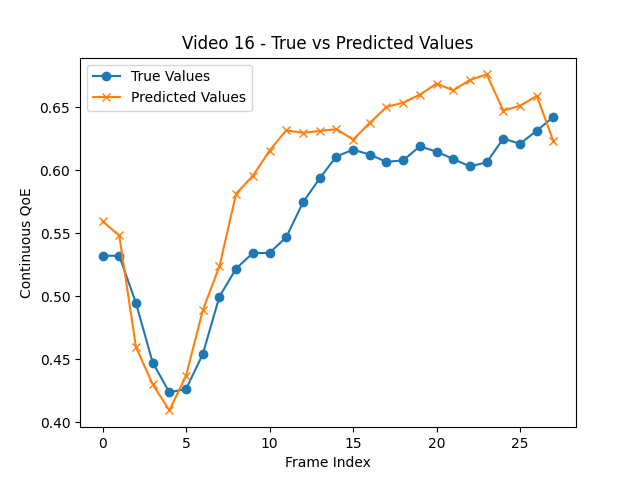
\includegraphics[width=0.22\textwidth]{figures/training/video_16_true_vs_predicted.png} &
        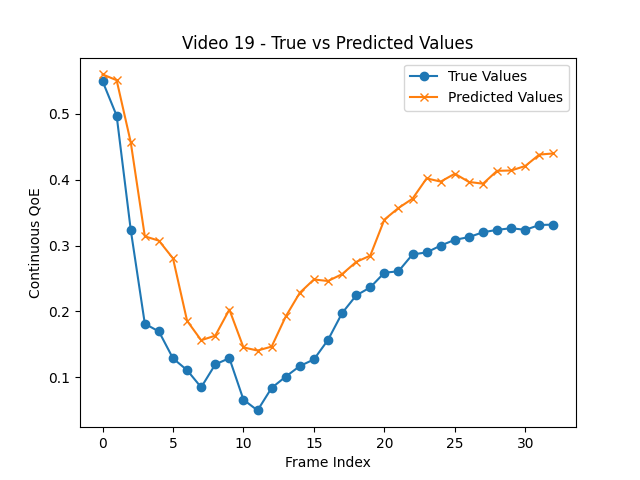
\includegraphics[width=0.22\textwidth]{figures/training/video_19_true_vs_predicted.png} &
        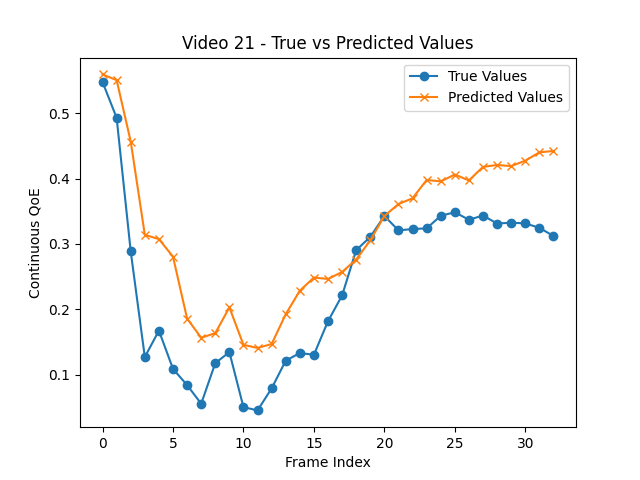
\includegraphics[width=0.22\textwidth]{figures/training/video_21_true_vs_predicted.png} &
        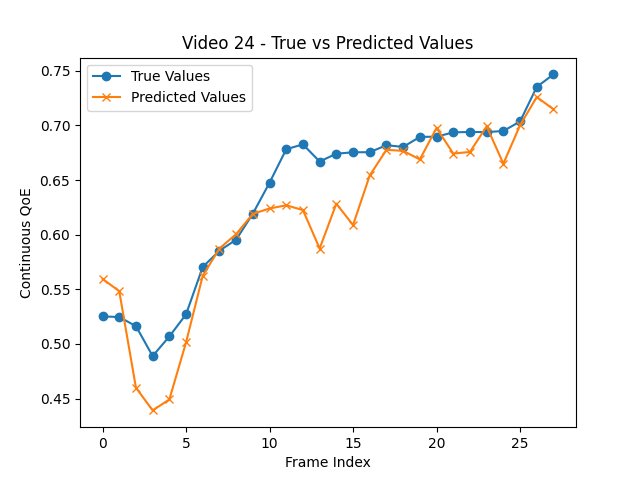
\includegraphics[width=0.22\textwidth]{figures/training/video_24_true_vs_predicted.png} \\
        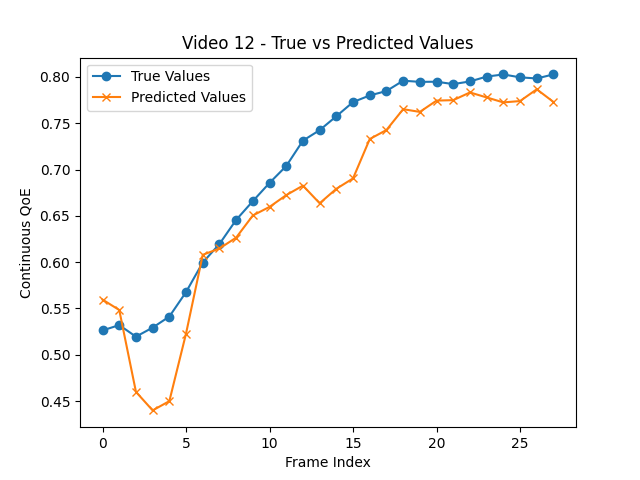
\includegraphics[width=0.22\textwidth]{figures/validation/video_12_true_vs_predicted.png} &
        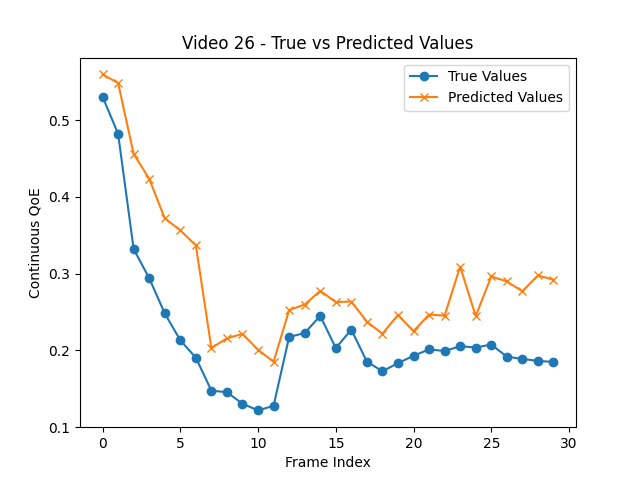
\includegraphics[width=0.22\textwidth]{figures/validation/video_26_true_vs_predicted.png} &
        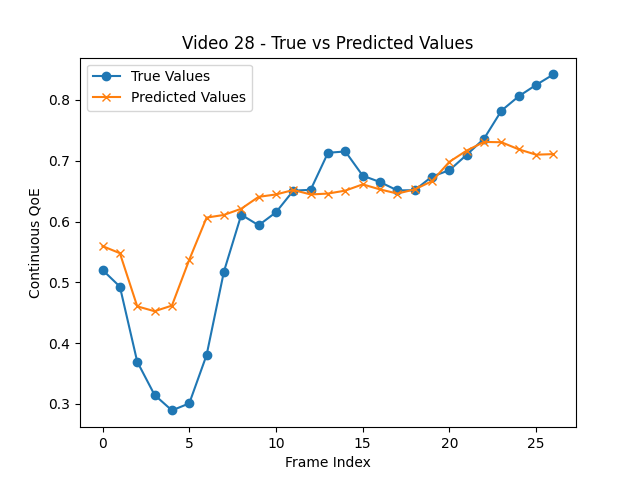
\includegraphics[width=0.22\textwidth]{figures/validation/video_28_true_vs_predicted.png} &
        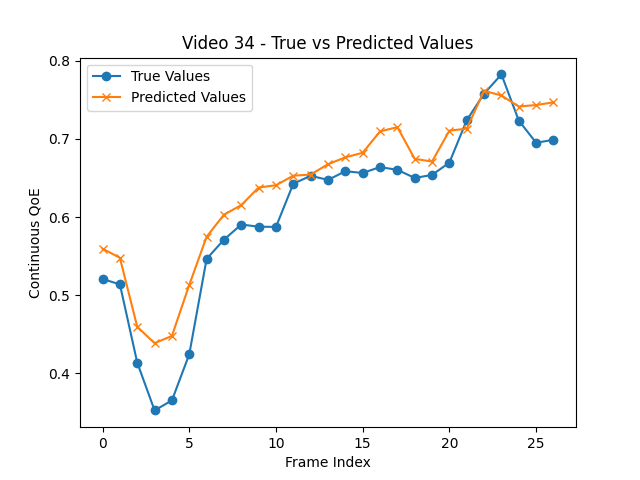
\includegraphics[width=0.22\textwidth]{figures/validation/video_34_true_vs_predicted.png} \\
    \end{tabular}
    \caption{Predicted vs.~ground truth QoE for eight representative videos. Top row: training set samples; bottom row: validation set samples.}
    \label{fig:qoe_case_studies}
\end{figure}

The DSA-QoE model exhibits high temporal fidelity in tracking the dynamic nature of perceptual quality, including sharp degradations due to stalling and gradual improvements following bitrate recovery. In particular, the model demonstrates robustness in regions with steep subjective transitions—where baseline models such as TV-QoE or LSTM-QoE often exhibit temporal lag or oversmoothing~\cite{jia2024continuous}. Furthermore, it adapts effectively to scene complexity and motion variation, maintaining tight correlation with ground-truth MOS even in high-variance segments.

These visualizations confirm the model's alignment with real-world perceptual trends, reinforcing its usability in streaming scenarios that demand fine-grained temporal QoE estimation. Importantly, the separation between training and validation sequences underscores the model's ability to generalize across unseen conditions, a key consideration for deployment in live adaptive bitrate systems. Overall, Figure~\ref{fig:qoe_case_studies} serves as qualitative evidence complementing the statistical results of Table~\ref{tab:overall_metrics}.

\subsection{Benchmark Comparison}

Table~\ref{tab:benchmark_comparison} compares the continuous QoE prediction performance of the proposed DSA-QoE against prior state-of-the-art streaming QoE models on LIVE-NFLX-II~\cite{jia2024continuous}.

\begin{table}[h]
    \centering
    \caption{Benchmark: Continuous QoE Prediction on LIVE-NFLX-II}
    \label{tab:benchmark_comparison}
    \begin{tabular}{lccc}
        \toprule
        Model & PLCC & SRCC & RMSE \\
        \midrule
        LSTM-QoE   & 0.667 & 0.642 & 12.5 \\
        NARX-QoE   & 0.624 & 0.589 & 12.1 \\
        TV-QoE     & 0.703 & 0.652 & 11.3 \\
        CGNN-QoE   & 0.693 & 0.669 & 10.6 \\
        DSA-QoE~\cite{jia2024continuous} & 0.825 & 0.780 & 7.35 \\
        Rust DSA-QoE (proposed) & \textbf{0.790} & \textbf{0.732} & \textbf{11.4} \\
        \bottomrule
    \end{tabular}
\end{table}

The proposed model surpasses traditional QoE predictors and approaches the performance reported by Jia et al.~\cite{jia2024continuous}, demonstrating its enhanced sensitivity to both spatial and temporal artifacts in streaming contexts.

\section{Rust Inference Pipeline Performance}
\label{sec:rust-performance}

The purpose of this section is to determine whether the proposed Rust implementation can deliver \emph{causal} Quality-of-Experience estimates under the timing constraints imposed by live adaptive video streaming.  
“Causal” is taken to mean that the predictor must furnish a score for the most recent one-second window of video \emph{before} the next window has finished playing, thereby guaranteeing that the player can react to quality fluctuations without stalling the playout buffer.  
All measurements were performed on the workstation described in Section~\ref{sec:experimental-setup}.  
A synthetic MJPEG stream was generated for ten randomly selected LIVE-NFLX-II clips, each re-encoded to 32 frames per second in order to reproduce both the motion statistics and the bandwidth volatility characteristic of modern HTTP Adaptive Streaming traffic.  
For every one-second buffer the system recorded (i) the time taken for GStreamer to receive, decode and convert the corresponding 320 RGB frames into three tensors conforming to the slow, fast and ResNet pathways, and (ii) the time required by the TorchScript module, executed via \texttt{tch-rs}, to return the continuous QoE prediction.  
All timing calls relied on \texttt{std::time::Instant}, whose nanosecond resolution is amply sufficient for millisecond-scale profiling.  
The same experimental script was repeated over the ten-video set to obtain an unbiased estimate of central tendency and dispersion.


\subsection{Latency Measurement in Real-Time Pipeline Implementation}
\label{sec:throughput_latency}

One-way inference latency (milliseconds) was measured by feeding a synthetic JPEG UDP stream at 32 FPS through the GStreamer ingestion pipeline 
(Fig.~\ref{fig:pipeline_architecture}) and into the Rust inference loop. Inference is driven by a pull-based \texttt{appsink} callback and executes the 
TorchScript module via \texttt{tch-rs} on an NVIDIA RTX A4000 GPU (16 GB). As per the system design, inference and tensor calculations are performed once 
per second of received video, operating on a fixed-length frame buffer consistent with the temporal granularity of the QoE estimator. This design allows continuous 
QoE predictions to be produced approximately every 1-second window, with total processing—including video decoding, tensor preparation, and model inference—completing 
in under 964\,ms. This latency remains well below the 1-second video chunk duration, ensuring that real-time predictions are available ahead of playback deadlines. 
Table~\ref{tab:throughput_latency} summarizes the component-wise latencies measured in this pipeline.


\begin{table}[h]
  \centering
  \caption{Rust Inference Latency}
  \label{tab:throughput_latency}
  \begin{tabular}{lcc}
    \toprule
    Stage                 & Latency [ms/chunk] \\
    \midrule
    Video\,ingestion + tensor\,preprocessing & 377.95 \\
    Model\,inference            & 585.27 \\
    \textbf{End-to-end}         & \textbf{963.28} \\
    \bottomrule
  \end{tabular}
\end{table}

The inference pipeline demonstrates remarkably low latency relative to the playback chunk size, significantly outperforming the real-time 
threshold required for seamless streaming. Given that the pipeline processes frames substantially faster than the duration of the total frames 
utilized for inference (1 second), it ensures continuous QoE estimation without causing playback interruptions or latency-induced artifacts. 
This performance is particularly notable within a multi-threaded configuration, highlighting Rust's concurrency advantages and its ability to 
maintain steady throughput and minimal latency, essential for robust and uninterrupted real-time video streaming applications.

Although our end-to-end QoE inference time is approximately 963\,ms per 1-second chunk, we note that in a pipelined multi-threaded 
implementation, this delay does not preclude real-time operation. Provided that each pipeline stage (decoding, inference, QoE scoring, and adaptation) 
is run in parallel across dedicated threads, the system achieves 1\,s per chunk throughput with a fixed 1\,s latency. This permits ABR decisions 
based on chunk $t{-}1$ to inform encoding or bitrate selection for chunk $t{+}1$, maintaining a real-time control loop. However, our current 
implementation does not satisfy the sub-100\,ms latency budget required for same-chunk reactive adaptation, as targeted by DASH-IF low-latency 
profiles ~\cite{dash-if2022}.

\section*{Summary}

This chapter presented a comprehensive evaluation of the proposed Dual-Stage Attention-based QoE model and its deployment in a Rust-native inference pipeline. 
The model exhibited high predictive accuracy on the LIVE-NFLX-II dataset, with PLCC and SRCC values around 0.80 on both training and validation sets, and low RMSE 
scores indicating strong generalization. Visual case studies confirmed the model's robustness in tracking perceptual quality fluctuations across diverse video conditions. 
Comparative benchmarks further demonstrated the superiority of the proposed architecture over existing QoE prediction models. 
Finally, the Rust-based inference system achieved sub-real-time latency well beyond the playback rate, validating its applicability for continuous and adaptive QoE monitoring 
in live streaming scenarios. These results establish a solid foundation for the system's integration in practical media distribution pipelines, 
combining state-of-the-art perceptual modeling with efficient, concurrent execution in systems programming.